\chapter{基础部分}
让你折腾完了你就得到了一个勉强能用的openSUSE
\section{安装openSUSE以及分区}
安装openSUSE请参见\href{https://zh.opensuse.org/%E6%96%B0%E6%89%8B%E6%9D%91}{新手村}。
另外本文主要针对安装了KDE桌面环境的openSUSE的用户,其他环境如GNOME下可能会有某些地方不同。注意,对于使用UEFI引导的电脑,只能使用DVD安装,具体可以参照\href{https://forum.suse.org.cn/viewtopic.php?f=2&t=802}{~Windows 8 (UEFI) 硬盘安装 openSUSE}

对于桌面用户,一般只需要\command{/, /home, swap}三个分区即可,分区大小与具体使用有关。\command{swap}分区相当于是虚拟内存,对于内存大的用户其实很少使用,但是如果你要使用休眠功能,则需要相应增大。\command{swap}的大小一般桌面用户可以用公式$y=\sqrt{x}\sim2\sqrt{x}$计算,其中$y$代表\command{swap}分区的大小,$x$代表内存大小,单位皆为GB。\command{/home}是你的家目录,用于存放你的各种文档视频等,如果你重装系统可以选择保留它以保存自己的一些数据等。它的大小较为随意,若在空间足够的情况下最好不小于50G。根分区\command{/}则主要取决于你安装的程序(它们会在\command{/usr}中),比如你安装了\textsc{Matlab}就会占用7.9G,而Mathematica 会占用约4.5G,如果你不要安装这类大型软件,可能30G足矣,而如果你要安装很多这种软件,那么至少要有50G的根分区空间。分区大小并没有严格的准则,可以视磁盘空间情况相应增大或者减少。
如果可能的话,为每个文件系统至少保留$25\%$的额外空间以应对今后的变化,还可以避免文件系统碎片。

对于密码,不要设的太复杂,不然每次安装软件都输一次密码将会很痛苦。当然,密码也是可以之后用\command{passwd}命令再修改的。
\section{基本概念}
\subsection{Linux的一些基本概念}
\paragraph{终端} Shell是各种命令的入口,而终端相当于是为Shell提供了一个图形界面,如KDE下面的\soft{konsole}。\emp{本文中大部分命令都是在终端中运行的。}

\paragraph{root权限} 顾名思义,root权限就是最根本权限。也就是说,有了root权限,你基本上有了做任何事的权力。
而执行某些命令,如安装、卸载软件包时需要root权限。此时你需要在命令前加sudo才能执行。
默认情况下输入密码时不会有类似于\command{****}的提示符。你也可以用su这个命令切换到root用户,
但是安全起见,在不必要的时候还是不要用su切换到root。\emp{注意,在命令行中以root权限打开相关图形程序时,需要使用\command{kdesu}来代替\command{sudo}!}

\paragraph{软件源} 软件源就是软件下载的来源。如果你已经添加的所有源里面都没有想要的软件包,但是在软
件包搜索或其他源中有,那你只需添加相应的源,再刷新源即可在\zy 中找到。添加软件源的方法可以参见\href{https://zh.opensuse.org/SDB:%E6%B7%BB%E5%8A%A0%E8%BD%AF%E4%BB%B6%E6%BA%90}{添加软件源}
%\item[依赖关系]
\subsection[包管理器]{openSUSE下的包管理器}
openSUSE下安装软件一般先用\zy 搜索,找到了便可以直接用\zy 安装。
如果搜索不到,说明你添加的的所有软件源里面都没有包含这个软件,此时你就需要用软件包搜索了。搜到了便一键安装,否则便只能采取最后方法——自行编译了。如果你你有打包能力并且这个程序不违反OBS相关规定,那么你就把它丢到OBS上面去,
然后别人也可以用这个打好了的包了。
\paragraph{zypper}\label{pre} 它是一个命令行的包管理器,常用命令有
\begin{Verbatim}[formatcom=\color{codec}]
    zypper update #升级软件包
    zypper refresh #刷新软件源
    zypper install PKG1 PKG2 #安装PKG1和PKG2等软件包
    zypper remove PKG1 PKG2 #移除PKG1和PKG2等软件包
\end{Verbatim}
其中上述选项都可以简化输入,对应关系为:
\begin{compactitem}
 \item \simp{update}{up}
 \item \simp{refresh}{ref}
 \item \simp{install}{in}
 \item \simp{remove}{rm}
\end{compactitem}

使用\command{in}选项时既可以安装源中的软件也可以安装当前目录下的rpm软件包。想要了解更多命令及其选项可以用\command{zypper --help}查看相关帮助。如果不想每次运行\zy (比如搜索软件包)的时候都自动刷新一次,你可以禁用所有软件源的自动刷新:
\begin{Verbatim}[formatcom=\color{codec}]
    zypper mr -Ra
\end{Verbatim}

\paragraph{YaST} 这相当于Windows中的控制面板,让你无需打开命令行即可在图形界面完成包括软件包管理、用户和组管理等在内的各种任务。在软件管理方面,你可以使用YaST直观的切换软件包的不同版本。
\begin{figure}[htbp!]
\centering
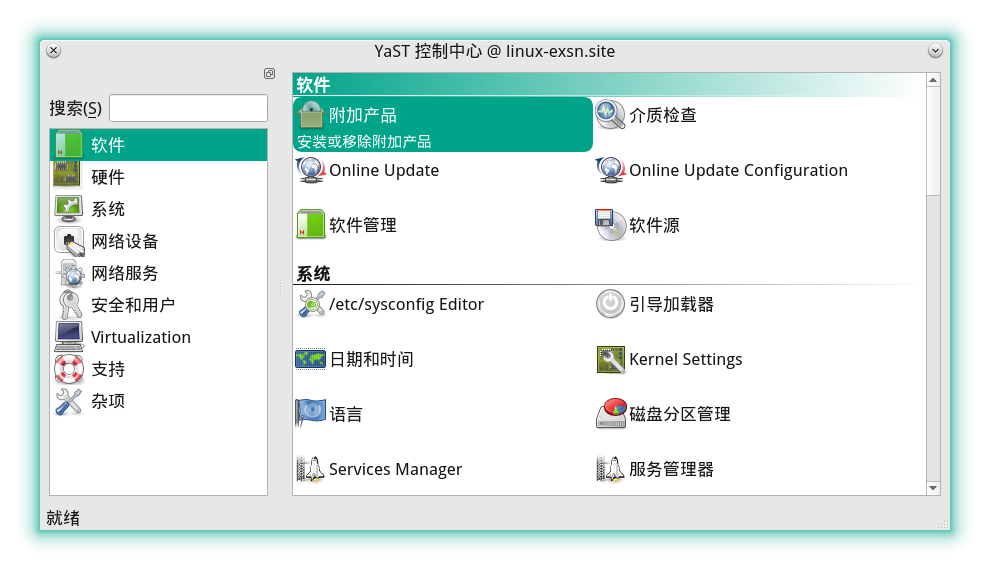
\includegraphics[width=\textwidth]{./pic/yast.png} 
\caption{YaST}\label{yast}
\end{figure}

\paragraph[软件包搜索与一键安装]{\href{http://software.opensuse.org/packages}{软件包搜索}与一键安装} 不同于Windows等操作系统,在Linux下大部分程序都是通过包管理器全局管理。所以安装软件在源中有该软件包的情况下只需要一个命令或用YaST的图形界面就可以搞定。如果源里面没有,那么在这里你可以搜索你想要的软件包。如果你利用\href{https://build.opensuse.org/}{OBS}编译了软件包,那么全世界的人都可以在这里使用它。
火狐浏览器自带了这个搜索引擎。在软件包搜索中找到软件以后,你就可以点击一键安装按钮了。一
键安装使得openSUSE中安装程序十分方便。在你进行软件包搜索后如果有多个源可以选择,同等条件下尽量选择
看起来比较官方的。\[\text{搜索软件}+\text{添加软件源}+\text{刷新软件源}+\text{安装软件}=\text{一条龙服务}\]

\begin{figure}[htb]
\centering
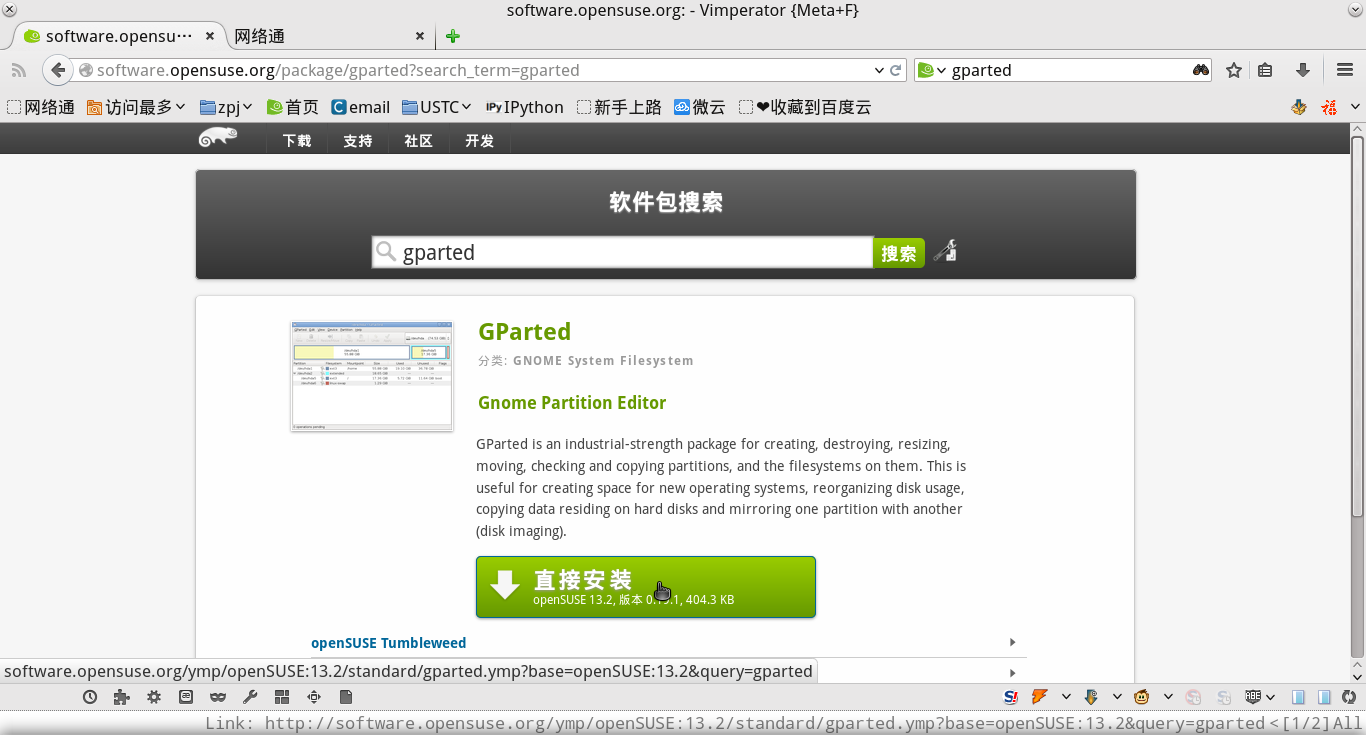
\includegraphics[width=\textwidth]{./pic/software.png} 
\caption{Firefox中的软件包搜索}\label{soft}
\end{figure}

\paragraph{常用软件源}\label{repo}

\begin{compactdesc}
 \item[\href{http://mirrors.hust.edu.cn/packman/suse/openSUSE_13.2/}{Packman}]
 提供多媒体编解码器、播放器、Broadcom无线网卡驱动、游戏等
 \item[\href{http://download.opensuse.org/repositories/home:/opensuse_zh/openSUSE_13.2/}{opensuse\_zh}]
 此软件源由中文用户维护,提供WPS等软件。
 \item[\href{http://download.opensuse.org/repositories/KDE:/Extra/openSUSE_13.2/}{KDE:Extra}]
 含有大量额外的KDE程序。
 \item[\href{http://download.opensuse.org/repositories/GNOME:/Apps/openSUSE_13.2/}{GNOME:Apps}]
 含有大量GNOME程序。
 \item[\href{http://dl.google.com/linux/chrome/rpm/stable/i386}{Chrome~32位}|\href{http://dl.google.com/linux/chrome/rpm/stable/x86_64}{64位}] 含有各种稳定版及非稳定版的Google Chrome
\end{compactdesc}
\subsection{KDE下寻找程序的方法}
如果你没有将程序的图标添加到桌面,那么你可以通过以下方法寻找并启动它。
\paragraph{启动器} 全称Kickoff应用程序启动器,是类似于Windows中“开始菜单”的一个东西,一般可以用Alt+F1调出。
新安装的程序可能暂时无法从这里启动。
\begin{figure}[htbp!]
\centering
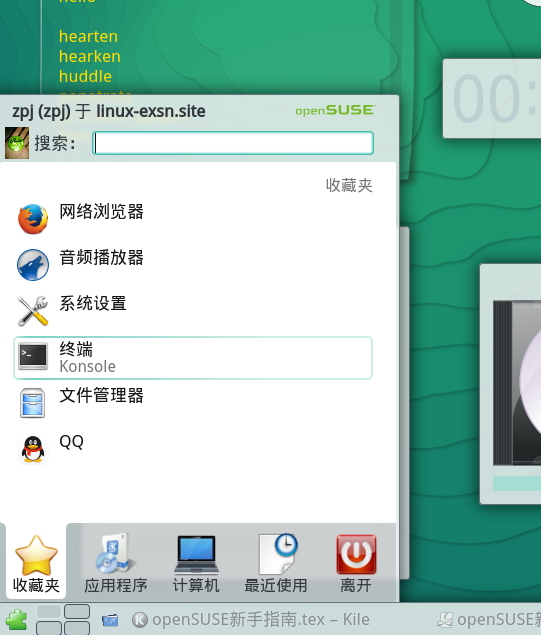
\includegraphics[width=0.9\textwidth]{./pic/kickoff.png} 
\caption{Kickoff应用程序启动器}
\end{figure}

\paragraph{Krunner} 是类似于Windows中的“运行”的一个东西,一般可以用Alt+F2调出,之后输入你要运行或要搜索的程序即可。
\begin{figure}[htbp!]
\centering
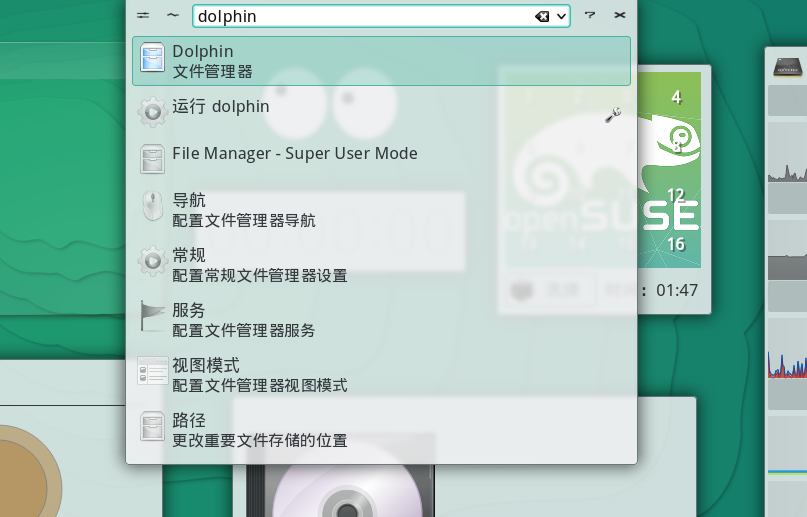
\includegraphics[width=\textwidth]{./pic/krunner.png} 
\caption{Krunner}
\end{figure}
\section{更新系统}
为了使你的更新过程尽可能块,你可能需要添加镜像源,比如中国科大镜像,可以参考相
应的\href{https://lug.ustc.edu.cn/wiki/mirrors/help/opensuse}{镜像使用帮助}之
后,按照提示添加并刷新软件源。但是使用镜像源有可能会由于镜像源和官方源没有完全同步,导致一直提示无法下载相应的软件包,这时你只能稍后再更新。

之后你就可以在终端中输入\command{sudo zypper up}更新系统了,这是很重要的一步。

运行\zy 进行软件管理时,经常会由于系统后台正在运行一个zypper(系统只能同时运行一个zypper),影响你添加软件源等各种操作。你可以在终端中输入\command{sudo kill pid}把这个进程杀掉,pid是它的进程号。

刷新软件源时有时候会出现网络故障或者源的故障导致无法刷新,解决方法就是检查网络以及源的可用性,如果不可用就换其他镜像或者使用官方源。

由于openSUSE中可能有一个软件包的不同厂商的版本,而openSUSE具有厂商黏性,因此运行更新的时候常常会遇到类似的情况:“将不会安装以下 51个软件包的更新:amarok apper bbswitch\ldots”,若对此有疑问请参见\href{https://forum.suse.org.cn/viewtopic.php?t=2777&p=21896}{为什么有些包不会被更新}
\section[双显卡]{双显卡关闭独立显卡}
\paragraph{NVIDIA} 如果你的显卡支持Bumblebee,请参见\href{https://zh.opensuse.org/SDB:Bumblebee}{SDB:Bumblebee},建议新手只安装bbswitch(不需要安装驱动),这样你可以直接跳过下一段。

如果你要安装bumblebee,建议采取加源安装方法。如果你要安装bumblebee
下载驱动时如果速度较慢,可以先用其他手段下载好,当安装到一半时按一次Ctrl+C,再将它替换掉\command{/usr/src/}下面的同名的\command{.run}文件,再在终端的问答中用r选项继续即可安装。如果安装到一半(驱动没有下载完整)使,按了两次Ctrl+C完全退出,那么会出现校验码不符合的错误,解决它的方法就是将\command{/usr/src/}下面的\command{.run}文件删除或替换为完整的驱动。

\paragraph{AMD} 如果你用的是开源驱动的话,在\command{/etc/init.d/after.local}后面加下面两行,那么开机后将会自动运行以关闭独显:
\begin{Verbatim}[formatcom=\color{codec}]
    echo IGD > /sys/kernel/debug/vgasitcheroo/switch
    echo OFF > /sys/kernel/debug/vgasitcheroo/switch    
\end{Verbatim}
具体请参考\href{https://linuxtoy.org/archives/how-to-use-vga-switcheroo-disable-video-card-linux-kms.html}{关闭独立显卡}。需要注意的是openSUSE并没有\command{/etc/rc.local}文件!你应该用类似于前述的\command{after.local}的文件代替。 

\section{中文环境的配置}
用LiveCD安装,无法得到完整的中文KDE环境,所以你需要安装
\begin{Verbatim}[formatcom=\color{codec}]
    kde4-l10n-zh_CN translation-update-zh_CN yast2-trans-zh_CN
\end{Verbatim}

为解决zip压缩包解压后文件名乱码的问题,请安装\soft{unzip-rcc}。

Fcitx是一个中文输入法框架,它对应的包为\soft{fcitx fcitx-config-kde4 fcitx-qt5\footnote{为了能够在QtCreator等程序中能够输入中文}}。安装好后再启动它,从此你的openSUSE就可以输入中文了。
装好后它的默认词库还很弱,你可以安装一个比较大的词库(非必需)。可%
以参见\href{https://code.google.com/p/hslinuxextra/}{hs\-linux\-extra}以及%
\href{https://www.librehat.com/fcitx-sogou-pinyin-cell-database-convert-import-guide/}{词库教程}%
或者下载我编译好的\href{http://pan.baidu.com/s/1i3HtJ4T}{pyphrase}文件,复制
到家目录的\command{.config/fcitx/pinyin/}中。
\begin{figure}[htbp!]
\centering
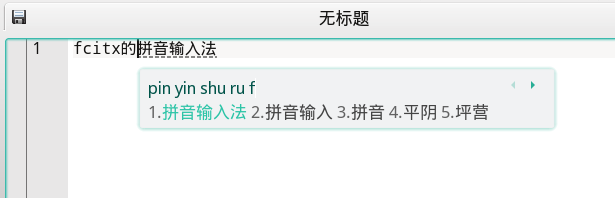
\includegraphics[width=\textwidth]{./pic/fcitx.png} 
\caption{输入法}\label{fcitx}
\end{figure}

当然你也可以不使用默认的拼音输入法而使用Fcitx的lib\-pin\-yin、谷歌拼音、搜狗拼音等输入法模块。对于大部分输入法你都可以使用云拼音(\soft{cloud\-pin\-yin})等模块。
安装好云拼音以后,只要在Fcitx的附加组件设置中配置好,你的输入法就可以利用云拼音输入了。注意,某些云拼音来源
可能会失效,如果云拼音无法使用可能就是因为这个原因。

其他输入法可能没有记忆学习功能,因此不能记录你的输入记录等,所以最好使用\emp{拼音}输入法+一个较好的词库+云拼音。
